In this section, we focus on the Phrase I of HTL and introduce our biased regularization for binary LS-SVM for our problem. Inspired by previous work, we bring a new perspective to the previous work and analysis the reasons why negative transfer could happen.

We define our transfer task in the following way: Suppose we have $N$ visual categories. 
In our source task, $N$ source binary classifiers $f'_n(x)$ for $n=1,...,N$, are trained from a distribution $\mathcal{D}_s$ to distinguish whether an object belongs to each of the $N$ categories. In our target task, we have another small set of data $(x,y)$ drawn from another distribution $\mathcal{D}_t$ with the same $N$ categories as those in source task. We want to train $N$ target binary classifiers $f_n(x)$ for $n=1,...,N$ on the data of the target domain so that they can perform well on the target domain.

\subsection{Biased regularization in HTL}
From previous works of HTL, the source and target classifiers $f$ follow the hypothesis space of all linear model, i.e. $f_n = w\phi(x)+b$, where $\phi(x)$ can be any feature mapping that maps the example into another space. The transfer learning process of each target binary classifier $f_n$ can be formalized as the following optimization problem:
\begin{equation}\label{eq:svm_obj}
\begin{aligned}
\textbf{min} && R({w_n}) + \frac{C}{2}\sum\limits_i^l {\mathcal{L}(f_n(x_i),Y_{in})} \\
\end{aligned}
\end{equation}
Here $R({w})$ is the regularization term to guarantee good generalization performance and avoid overfitting. $Y_{in}$ is the encoded label for binary classifier following $Y_{in}=1$ if $y_i=n$ and $-1$ otherwise. $\mathcal{L}(\cdot)$ is the loss function. When we consider to use Lease Square SVM as the classifier, $\mathcal{L}(f,y) = (f-y)^2$. 

In previous works, such as Multi-KT \cite{tommasi2014learning} , assume that the hyperplane $w_n$ of the target classifier should be closed to the weighted combination of the hyperplane of the source models. The optimization problem \eqref{eq:svm_obj} can be written as:
\begin{equation}\label{eq:opt}
\begin{aligned}
\textbf{min} \qquad & \frac{1}{2}{\left\| {{w_{n}} - \sum\limits_{k = 1}^N {w{'_k}{\beta _k}} } \right\|^2} + \frac{C}{2}\sum\limits_i^l {{e_{in} ^2}}\\
\textbf{s.t.} \qquad &  e_{in} = Y_{in}-w_n\phi(x_i)-b_n
\end{aligned}
\end{equation}

The optimal solution to problem (\ref{eq:opt}) is:
\begin{equation}\label{eq:solu}
\begin{aligned}
{w_{n}}&= \sum\limits_k^N {{\beta _k}{{w'}_k}}  + \sum\limits_i^l {{\alpha _{in}}{\phi(x_i)}} 
\end{aligned}
\end{equation}
It is obviously that once we can determine the values of the weights $\beta$, we can solve the optimization problem \eqref{eq:opt}.

\subsection{Data Augumentation in HTL}
We can interpret Eq. \eqref{eq:solu} in the following way. Let $w''_n=\sum\limits_i^l {{\alpha _{in}}{\phi(x_i)}}$, we have $w_{n} = w_{n}''+\sum\limits{\beta _kw'_k}$. Therefore, for the target binary classifier $f_n(x)$, we have:
\begin{equation}\label{eq:aug_pre}
\begin{aligned}
f_n(x)&=w_{n}''\phi(x)+\sum\limits_k^N{\beta _kw'_k\phi(x)}+b_n\\
&=w_{n}''\phi(x)+(b_n-\sum\limits_k^N{\beta _kb_k})+\sum\limits_k^N{\beta _kf'_k(x)}
\end{aligned}
\end{equation}
\begin{figure*}
\centering
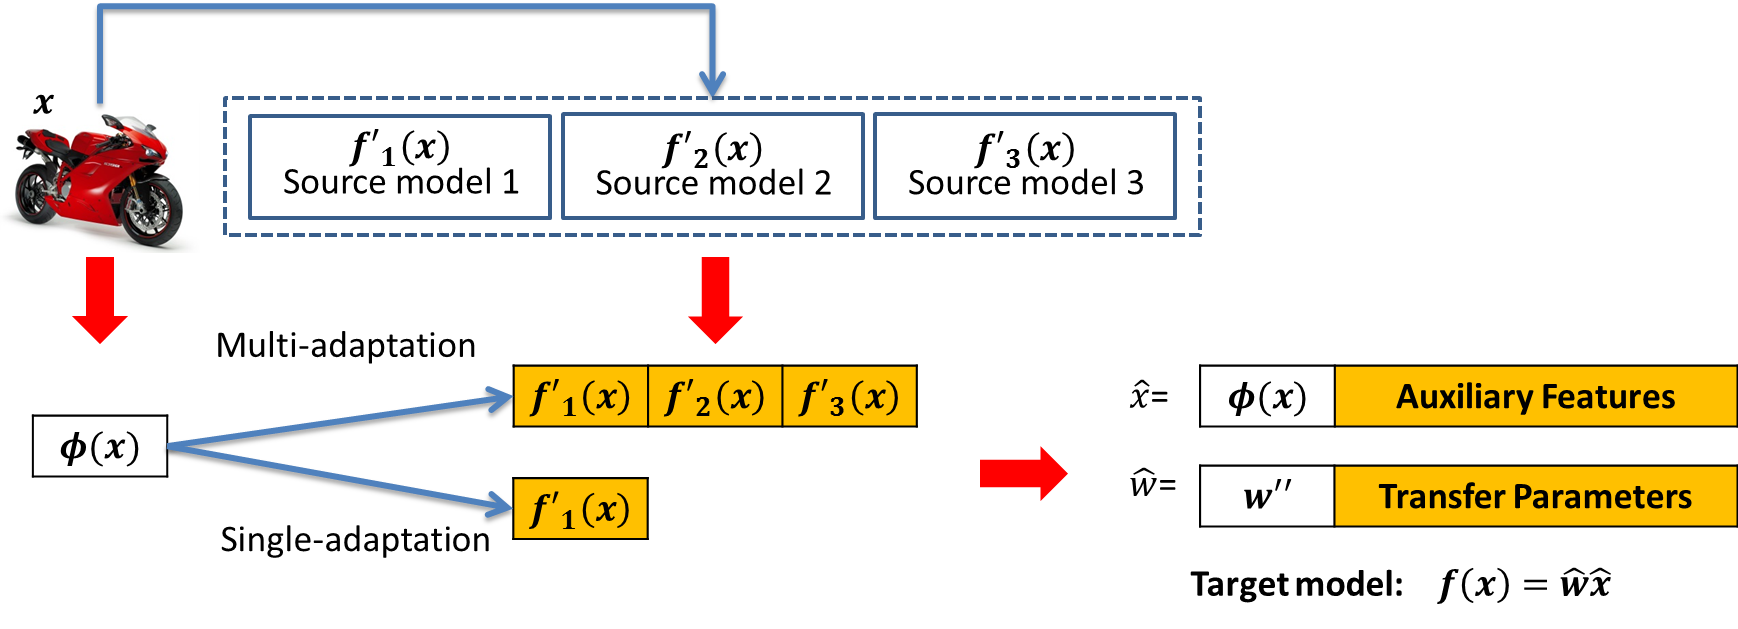
\includegraphics[scale=0.7]{fig/aug2.png}
\caption{The transfer learning process can be considered as the augmentation of the target data where the decision scores of the source models are appended as the auxiliary features. The transfer parameters can be considered as the a part of the corresponding hyperplane. We can consider 2 augmentation strategies: multi-adaptation and single-adaptation.}\label{fig:aug}
\end{figure*}
Here, we call the weight $\beta_k$ the transfer parameter. From Eq. \eqref{eq:aug} we can see that the decision of each target binary classifier is made by combining the decision from target task $w_{n}''\phi(x)$ and the decision scores of the source model. The transfer parameters here is to control the amount of the knowledge transferred from the source models.

We can rewrite Eq. \eqref{eq:aug_pre} as:
\begin{equation}\label{eq:aug}
\begin{aligned}
f_n(x)&= [w_{n}'',\beta_1,...,\beta_N][\phi(x),f'_1(x),...,f'_N(x)]^T\\&+(b_n-\sum\limits_k^N{\beta _kb_k})
\end{aligned}
\end{equation}
Here, we propose a novel insight to the transfer problem. From Eq. \eqref{eq:aug}, we can see that solving the optimization problem \eqref{eq:opt} is equivalent to find the optimal hyperplane $\hat{w}=[w_{n}'',\beta_1,...,\beta_N]$ for the augmented data $\hat{x}=[\phi(x),f'_1(x),...,f'_N(x)]$. An intuitive interpretation of the auxiliary feature is that it can be considered as a similarity score from the source model. When the target model decides whether an object belongs to certain category, it also weight the decisions of the source model as the reference.
Moreover, we can see that because the auxiliary features come from the decision scores of the source models, we can greatly extend the choice of the types of the source classifier. We can exploit the knowledge of any source model that can output the decision score of an example while previous methods are limited to SVMs \cite{tommasi2014learning} \cite{kuzborskij2013n}. When there are multiple source models, we can choose multiple sources (multi-source adaptation) or the best source (single-source) to augment the original data (see Figure \ref{fig:aug}).



\subsection{Reasons for negative transfer}
From the perspective of the feature augmentation, we can turn the problem of domain adaptation problem with HTL into a traditional learning problem, i.e. find the optimal values for the elements of the hyperplane hyperplane $\hat{w}=[w_{n}'',\beta_1,...,\beta_N]$. According to the principle of Structural Risk Minimization (SRM) \cite{vapnik1999overview}, the risk of a linear classifier $f(x)=wx+b$ on the unseen test data $R(f)$ (generalization risk) is bounded by:
\begin{equation}\label{eq:srm}
R(f) \le {R_{emp}}(f) + \sqrt {\frac{{h(\ln (2l/h) + 1) + \ln (\delta /4)}}{l}} 
\end{equation}
Here the first part on the right-hand side of the inequation ${R_{emp}}(f)$ is the empirical risk (training error) of the classifier and the second part is the confidence interval. $h$ and $l$ denote the VC dimension and number of training data of the classifier respectively and $\delta$ is the confidential parameter. According to \cite{suykens1999least}, the VC dimension $h$ is bounded by $h \le \min([||w||^2R^2],l)+1$ where $R$ is the radius of the smallest ball containing data $x$ and $||w||$ is the \textit{2-norm} of the hyperplane.

As we discussed above, we use the outputs of the source models as the auxiliary features to augment the target data. Let $R$ and $\hat{R}$ denote the radius of the data before and after augmentation. We should have $R^2 \le \hat{R}^2$ and $||w||^2\le ||\hat{w}||^2$. This indicates that the VC dimension of the target model trained on the augmented data (augmented model) tends to increase compared to the model trained from the original data, i.e.  the method without transferring any source knowledge (no transfer model). As a result, feature augmentation eventually increases the confidence interval of the risk of the augmented model. When the augmented model failed to decrease the empirical risk, its performance would degrade, i.e. suffer from negative transfer. For example, when the auxiliary features can't provide any extra useful information for classification, i.e. the source domain and target domain are unrelated, negative transfer could happen. In contrast, if we can significantly decrease the empirical risk of the augmented model, we can decrease its generalization risk and get improved performance, i.e. positive transfer.

From the analysis above, we can see that in order to get improved performance and alleviate negative transfer, we have to carefully control the value of the transfer parameters. A naive method to estimate the hyperplane $\hat{w}$ for the target model could be following the idea of optimizing problem \eqref{eq:svm_obj} to minimize the training error of $f(x)=\hat{w}\hat{x}+b$ directly. However, if we are not able to regularize the transfer parameters properly, the target model could easily suffer from negative transfer when the source and target are weakly related (see the experiments in Section sec:exp).
In next section, we introduce our method SMTLe to estimate the transfer parameters that can improve the performance of the target model and alleviate negative transfer .

